\documentclass[11pt]{article}
\addtolength{\oddsidemargin}{-1.cm}
\addtolength{\textwidth}{2cm}
\addtolength{\topmargin}{-2cm}
\addtolength{\textheight}{3.5cm}

\usepackage[pdftex]{graphicx}
\usepackage{pdflscape}
\usepackage{hyperref}
\usepackage{float}
\usepackage{cite}
\hypersetup{
	colorlinks=true,
	linkcolor=black,
	filecolor=magenta,
	urlcolor=cyan,
}

% define the title
\author{Team C\#}
\title{Architectural Requirements Specifications and Design for the NavUP System}

\begin{document}
	\setlength{\parskip}{6pt}
	
	% generates the Cover page
	\begin{titlepage}
	\begin{center}
		% Upper part of the page       
		
\includegraphics[width=0.7\linewidth]{uniLogo.jpg}\\[1cm]    
		\textsc{\LARGE Team C\# Round 2}\\[0.3cm]
		% Title
		\rule{\linewidth}{0.5mm} \\[1cm]
		{ \huge \bfseries Architectural Requirements Specifications and Design for the NavUP System}\\[0.5cm]
		\rule{\linewidth}{0.5mm} \\[1cm] 			
		
		\begin{minipage}{0.4\textwidth}
			\begin{flushleft} \large
				Peter {Boxall}
			\end{flushleft}
		\end{minipage}
		\begin{minipage}{0.4\textwidth}
			\begin{flushright} \large
				\emph{} \\
				U14056136 
			\end{flushright}
		\end{minipage}
		
		
		\begin{minipage}{0.4\textwidth}
			\begin{flushleft} \large
				\emph{} \\
				Seonin {David}
			\end{flushleft}
		\end{minipage}
		\begin{minipage}{0.4\textwidth}
			\begin{flushright} \large
				\emph{} \\
				U15063021
			\end{flushright}
		\end{minipage}
		
		
		\begin{minipage}{0.4\textwidth}
			\begin{flushleft} \large
				\emph{} \\
				Mia {Gerber}
			\end{flushleft}
		\end{minipage}
		\begin{minipage}{0.4\textwidth}
			\begin{flushright} \large
				\emph{} \\
				U15016502
			\end{flushright}
		\end{minipage}

		\begin{minipage}{0.4\textwidth}
			\begin{flushleft} \large
				\emph{} \\
				Keamogetswe {Matsobe}
			\end{flushleft}
		\end{minipage}
		\begin{minipage}{0.4\textwidth}
			\begin{flushright} \large
				\emph{} \\
				U16087004
			\end{flushright}
		\end{minipage}

		\begin{minipage}{0.4\textwidth}
			\begin{flushleft} \large
				\emph{} \\
				Oratile {Motswagosele}
			\end{flushleft}
		\end{minipage}
		\begin{minipage}{0.4\textwidth}
			\begin{flushright} \large
				\emph{} \\
				U15306195
			\end{flushright}
		\end{minipage}

		\begin{minipage}{0.4\textwidth}
			\begin{flushleft} \large
				\emph{} \\
				Banele {Nxumalo}
			\end{flushleft}
		\end{minipage}
		\begin{minipage}{0.4\textwidth}
			\begin{flushright} \large
				\emph{} \\
				U12201911
			\end{flushright}
		\end{minipage}

		\begin{minipage}{0.4\textwidth}
			\begin{flushleft} \large
				\emph{} \\
				Craig {van Heerden}
			\end{flushleft}
		\end{minipage}
		\begin{minipage}{0.4\textwidth}
			\begin{flushright} \large
				\emph{} \\
				U15029779
			\end{flushright}
		\end{minipage}
		
	\end{center}
\end{titlepage}
	
	\tableofcontents
	
	\newpage
	
	\section{Deployment Diagram}
	\begin{figure}[H]
		\centering
		\includegraphics[scale=0.54]{deployment_diagram.png}
		\caption{Deployment Diagram}
		\label{fig:deployment_diagram}
	\end{figure}
	
	\newpage
	
	\section{Fitness Module}
	\subsection{Design Constraints}

\subsubsection{Software Constraints}
\begin{enumerate}
	\item Device Accelerometer Support:
	\newline
	Given that a device does has an accelerometer, the device manufacturer must provide a software interface to interact with the device's accelerometer.
\end{enumerate}

\subsubsection{Hardware Constraints}
\begin{enumerate}
	\item Accelerometer:
	\newline
	Not all devices models are made equal. Some older devices do not have accelerometers to track steps with. The accuracy of accelerometers also vary from different device manufacturers.
	\item Battery Life:
	\newline
	To track steps continuously with a background process will greatly impact the battery life of devices with small battery capacities. 
\end{enumerate}

\subsection{Software System Attributes} 
\subsubsection{Reliability} 
The fitness module must be able to accurately and reliably track movement through the devices accelerometer. This accuracy and reliability ensures that the calculation of steps, calories and other health related data is accurate. The accuracy and reliability requirements are to ensure that milestones and awards are distributed accurately.    

\subsubsection{Efficiency} 
In order for the application to efficiently count steps and calculate other health metrics, the fitness module needs efficient algorithms to calculate the steps and other health metrics quickly from the data it recives from the accelerometer.  

\subsubsection{Portability} 
The fitness module should be able to work on both iOS and Android devices. There should also be no discernible differences between the fitness module on iOS and the fitness module on Android devices. They should also yield the same the same health metrics. 

\subsubsection{Coupling} 
The fitness module should also integrate with the user module. It should be able to request the users age and name. The fitness module should also be able to write data such as the users height and weight. Minimal helth metrics should also be sent to the user module to be stored on the server. 


\subsection{Activity Diagram}
See figure~\ref{fig:fitness_activity_diagram} on page~\pageref{fig:fitness_activity_diagram}
\begin{figure}
	\centering
	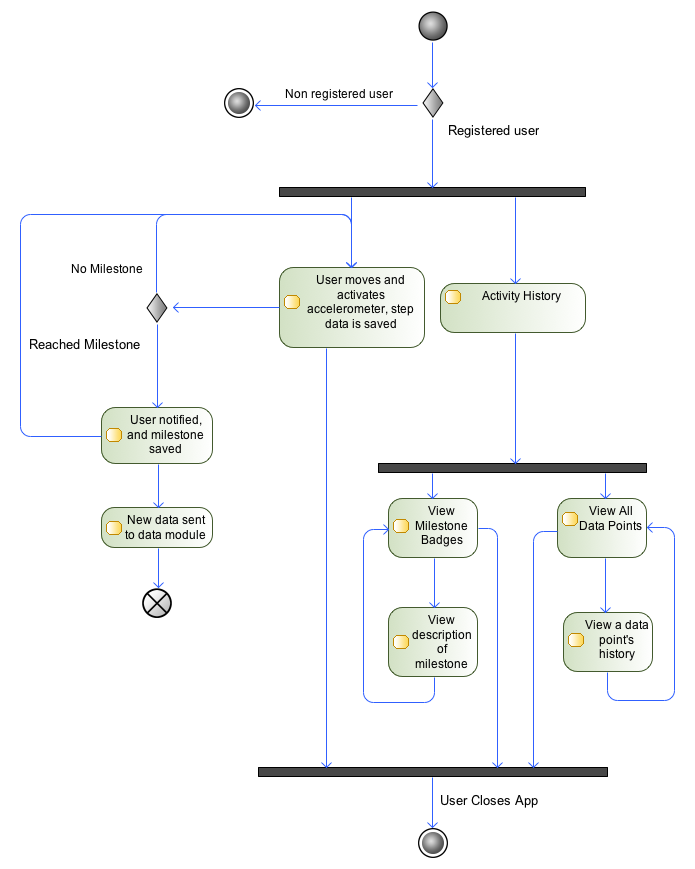
\includegraphics[scale=0.54]{Fitness/fitness_activity_diagram.png}
	\caption{Fitness Activity Diagram}
	\label{fig:fitness_activity_diagram}
\end{figure}

\subsection{State Diagrams}
See figure~\ref{fig:fitness_state_diagram} on page~\pageref{fig:fitness_state_diagram}
\begin{figure}
	\centering
	\includegraphics[scale=0.54]{Fitness/fitness_state_diagram.png}
	\caption{Fitness State Diagram}
	\label{fig:fitness_state_diagram}
\end{figure}
	
	\newpage
	
	\section{Navigation Module}
	\documentclass[a4paper,12pt]{article}
\usepackage{array}
\newcolumntype{L}{>{\centering\arraybackslash}m{8cm}}

%	Mia Gerber 
%	15016502
%	
%	COS 301: Assignment 2
%
%	Navigation Subsystem: Requirements, Constraints and Attributes

\begin{document}
	\newpage
	\section{Navigation}
	
	\subsection{External Interface Requirements}
	 \textbf{ \paragraph These requirements relate to both interfacing with other subsystems within the UP Nav system as well as interfacing with the hardware that the application will be deployed on.}
	\begin{itemize}
		\small
		\item To "Notifications" module will be used to give directions to the user during navigation in the form of push notifications.
		\item The "Points of interest" module will be seen by the Navigation module simply as destinations to be navigated to or as a current location.
		\item The GIS module will be used continually throughout navigation and as such is included in most of the UML diagrams, because of this tight coupling, implementation of the system needs to be done in a way that ensures easy communications between these two subsystems.
		\item Interfacing with the user's mobile device will be done with a cross platform API, explained in the "Technologies" section.
	\end{itemize}
	
	\subsection{Performance Requirements}
	\begin{itemize}
		\small
		\item Immediate response in the form of a notificaiton if user goes off route
		\item User can choose if application can continue navigation in the background even if the application isn't currently open. (Optional background data usage)
		\item "Fuzzy searching" when user is looking for a destination and misspells a word the application can still recognise the intended destination and navigate to the correct place.
		\item Navigation seamlessly continues when user suddenly changes from using campus wifi to using mobile data. (Interaction between GIS module and Navigation module is important here.)
	\end{itemize}
	
	\subsection{Design Constraints}
	\begin{itemize}
		\small
		\item The use of design patterns is crucial to object oriented software engineering but we are limited 
			in the types of design patterns we are able to use within the subsystems due to the requirements 
			imposed upon the system as a whole.
		\item The Navigation subsystem receives critical information from the GIS subsystem to ensure that the route
			calculated is correct and to recalculate the route in real time if the user goes off track. The coupling between these two modules will be high and might affect the implementation of other subsystems that also rely upon GIS information.
		\item Our application will be deployed across multiple platforms using different GIS implementations forcing the Navigation module to be able to perform uniformly when receiving coordinates in different formats or encodings.
		\item Users will want to limit the amount of data transfer occurring when using the application, the only way to implement this is to restrict communication with the server and database which could impact navigation efficiency and user experience.
	\end{itemize}
	
	\subsection{Software System Attributes}
	\begin{itemize}
		\small 
		\item High cohesion with low coupling allowing for easy addition, removal or replacement of modules.
		\item Polymorphism will be implemented as means of specifying object behaviour when the user imposes restrictions upon the base behaviour of the object.
		\item All source files will be written in an Object Oriented capable language.
		\item We will need to interface with the user's device at a level capable of accessing push notifications and 
		 GIS data.
	\end{itemize}
	
	\subsection{Design Patterns used}
	\paragraph{Discussion of design patterns implemented in UML diagrams:}
		Memento: To save a route for future use
		
		Splitting the functions of the Navigation module essentially leaves us with two structures within the module. An internal state that is constantly changing as well as a means of navigations (different algorithms to achieve navigation to destination). Keeping this in mind I decided to use the State and Strategy design patterns, these design patterns both function on the same basic principal of modularity and separation of concerns. Additionally, because the Strategy design pattern represents what is essentially a list of directions, if the user decides to save their route so that they may return to it later, the Memento design pattern was included to ensure sensible safekeeping.
		
		There are three possible states, namely: "Navigation in progress", "Navigation has been violated" and "Navigation exited successfully". Each one of these states interacts with the chosen strategy in a different way. which is why there is aggregation between the State and Strategy classes.
		
		The Strategy class and its subclasses will deal with user constraints by keeping an array of said constraints and constructing a graph using information gathered from both the GIS Module as well as user input to ensure graph traversal will result in a desirable route. 
	
\end{document}

	
	\newpage
	
	\section{Points of Interest}
	\section{External Interface Requirements}
	\subsection{System Interfaces}
The NavUp systems’ interfaces include locating and retrieving site information (building names, addresses, etc.) based on the information retrieved from the Navigation module. The site information will be used for gathering and maintaining any information of interest with regard to the “searched” location. The acquired information about the location will be stored and pushed as a notification to the users’ interface where users can view and read it.
	\subsection{User Interfaces}
The system will allow users to find locations, so the route guidelines to the destination will be displayed on the users’ screen interface, route guidelines include a pin-point indicating users’ current positon, colored route path to the destination, and the pin-point indicating the destination. So, once the information of interest with regard to the location has been acquired, the information will be sent to the user as a notification, and the notification may be in a form of SMS, E-mail, or a push notification. The user will have an option to alter how the notifications are received, that is, either as an E-mail, push notification or an SMS.
	\subsection{Hardware Interfaces}
The Wi-Fi routers and mobile phones are the only primary hardware interfaces that may be required for the “points of interest” module. Mobile phones will be used for all the user interfaces and the functionality of the NavUp system and the Wi-Fi access points as a reference for detecting locations both indoors and outdoors.
	\subsection{Software Interfaces}
The NavUp will primarily run on mobile phones. Therefore, for compatibility requirements, the NavUp system should be hybrid, that is, it has to be compatible across most, if not all ranges of mobile smart phones and mobile operating systems, that is either Android OS, iOS, or Microsoft Windows. The system can also be web-based.
	\subsection{Communication Interfaces}
The system will frequently communicate with the campus map database, servers and the mobiles’ GPS to get locations and directions through Wi-Fi networking. Any acquired information of interest with regard to the desired location may be retrieved from the database through servers. The systems’ communication interface may also include web services.
	
	\begin{figure}[H]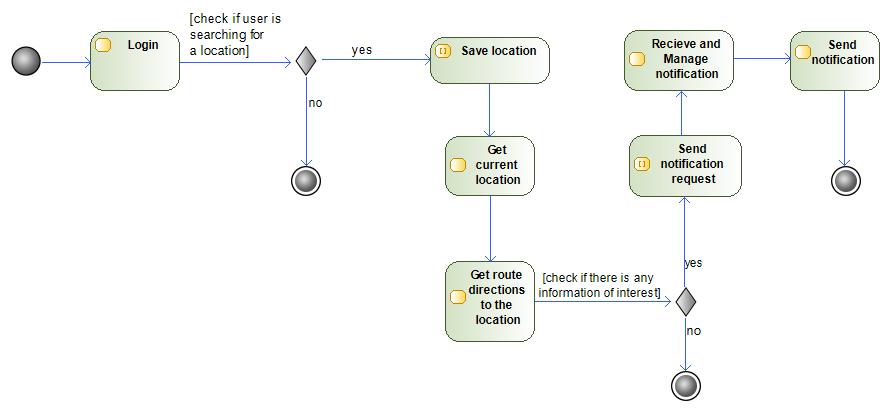
\includegraphics[width=\textwidth]{ActivityDiagram}
	\caption{UML Activity Diagram}
	\end{figure}
	
\section{Performance Requirements}
	\subsection{Track creation/ Route update}
	The NavUp system should also keep track of the user's current location
	so to update the route displayed on the user's screen interface, however 
	the system should not necessarily update the route every after 1 second, the 
	route update can be in an interval of 7 seconds per update.
	\subsection{User login response time}
	The users will be required to login, provided that the user has
	entered correct credentials, the NavUp system should take no longer
	than 6 seconds to provide full system access to the user. However, this
	may be dependent on the internet connection bandwith.
	\subsection{Positional accuracy}
	Accuracy is one of the vital performance required for the system. The NavUp 
	system should be accurate enough to get the user’s current position, if for 
	example the user is in the building (indoor) with multiple floors, the system 
	should not necessarily determine the exact venue, but it should be in range and 
	in real time.\\\\ The system should have a good ranging accuracy. The accuracy of the 
	system is defined as the solution error, and the accuracy of the system should conform 
	to position range and the PVT (Position, Velocity and Time). This will be useful in 
	terms of “points of interest” where accuracy is very important when determining locations.
	\subsection{Proximity of notifications}
	The user will recieve any information of interest for the locations he/she visits, the amount
	of time it takes to recieve the notification shouldn't be long, this is to say, the system should 
	be responsive enough to an extent that when the user gets to the desired location, it takes no longer 
	than 25 seconds to recieve the notification.
  
	\begin{figure}[H]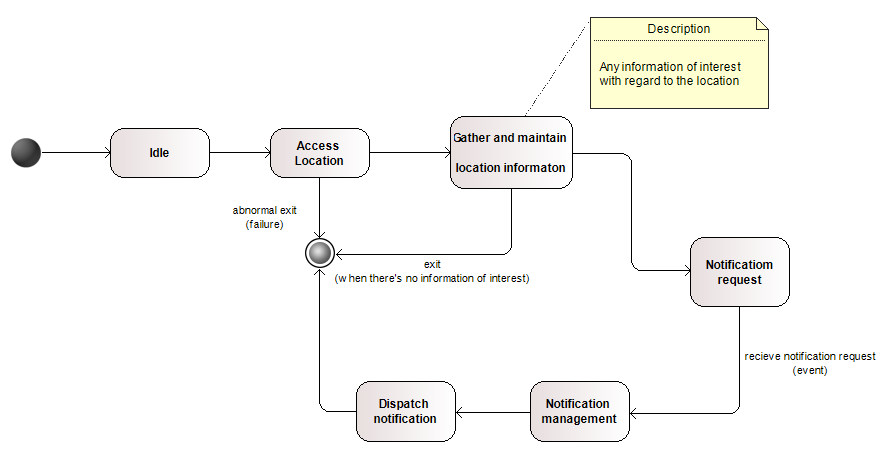
\includegraphics[width=\textwidth]{StateDiagram}
	\caption{UML State Diagram}
	\end{figure}
		
	\begin{figure}[H]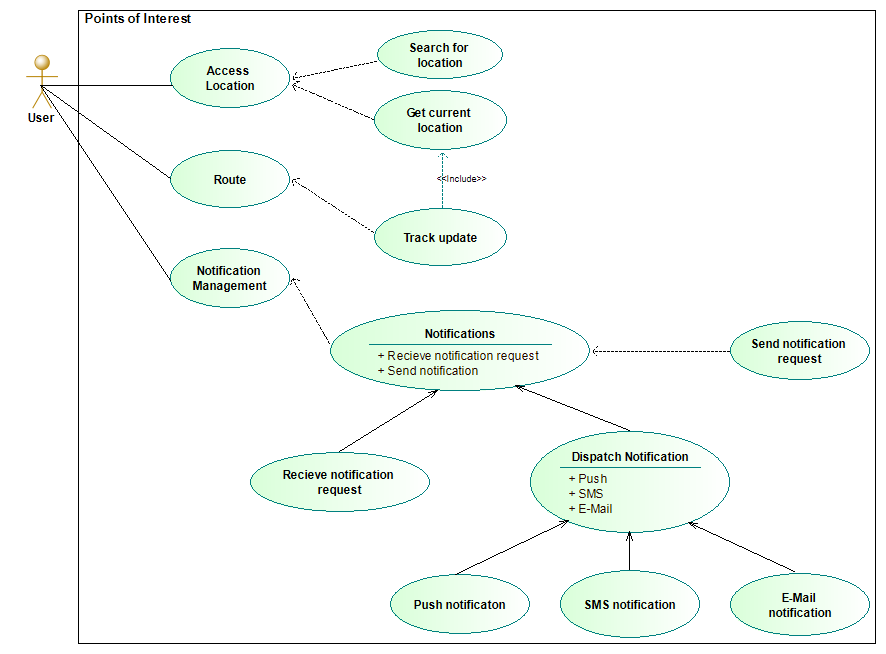
\includegraphics[width=\textwidth]{UseCaseDiagram}
	\caption{UML Use Case Diagram}
	\end{figure}

	
	\newpage
	
	\section{Users Module}
	\subsection{External Interface Requirements}
\begin{itemize}
	\item The user module interface will provide the user with a clean and smart design, which will make it easy for the user to access the system and logon or register with no unwanted constraints.
	\item The user will only be allowed to access his/her application via a smartphone or tablet. The software will work on any operating system. 
        \item The application will be able to fit all screen resolutions with screen rotation capabilities.
	\item When the user logs in or register, his/her information will be sent to a server which will then connect to a database that will either validate the user’s credentials or add the credentials to the system.
	\item To meet disability requirements, users can use the accessibility function that is built into almost all smartphones and tablets.
\end{itemize}
\subsection{Performance Requirements}
\begin{itemize}
	\item The user system will get from 20 000 to 40 000 login requests a day. This branches of into registered students logging into the system more than once a day and guests registering and logging into the system
	\item The user system will have at most 1000 guests using the application on the campus but this value varies in the beginning of the year because most first year have not registered within the first few weeks of the academic year. 
        \item The user system might slow down depending on how the database is implemented and how big it will be but the design patterns used help improve database efficiency and improves server response time.
\end{itemize}
\subsection{Design Constraints}
\begin{enumerate}
	\item Query caching
	\newline
	In order to avoid traffic requests to the database and to speed up database , query caching is crucial. AdoDB provides powerful caching system which can implemented in the navUP system and help improve speed regarding interaction between front end and database.
\end{enumerate}
\subsection{Software System Attributes}
\begin{enumerate}
	\item Security
	\newline
	The navUP system will need to adhere to the highest security standards because of the personal information of users that will be stored. In order to achieve security , The navUP system needs to store users’ information and the passwords should be stored in the database as encrypted to remain hidden from the unauthorised users  .
	\item Performance
	\newline
	The system should ensure that basic operations like user registration , user login should be of maximum speed. 
	\item Availability
	\newline
	The navUP system will need to be connected to the internet to ensure that the system can communicate with  the database.
	\item Reliability
	\newline
	The navUP system will need to work roburstly without any failures including failure to retrieve information from the database.
\end{enumerate}
\subsection{UML diagrams}
\subsubsection{Class diagram}
\begin{figure}[H]
	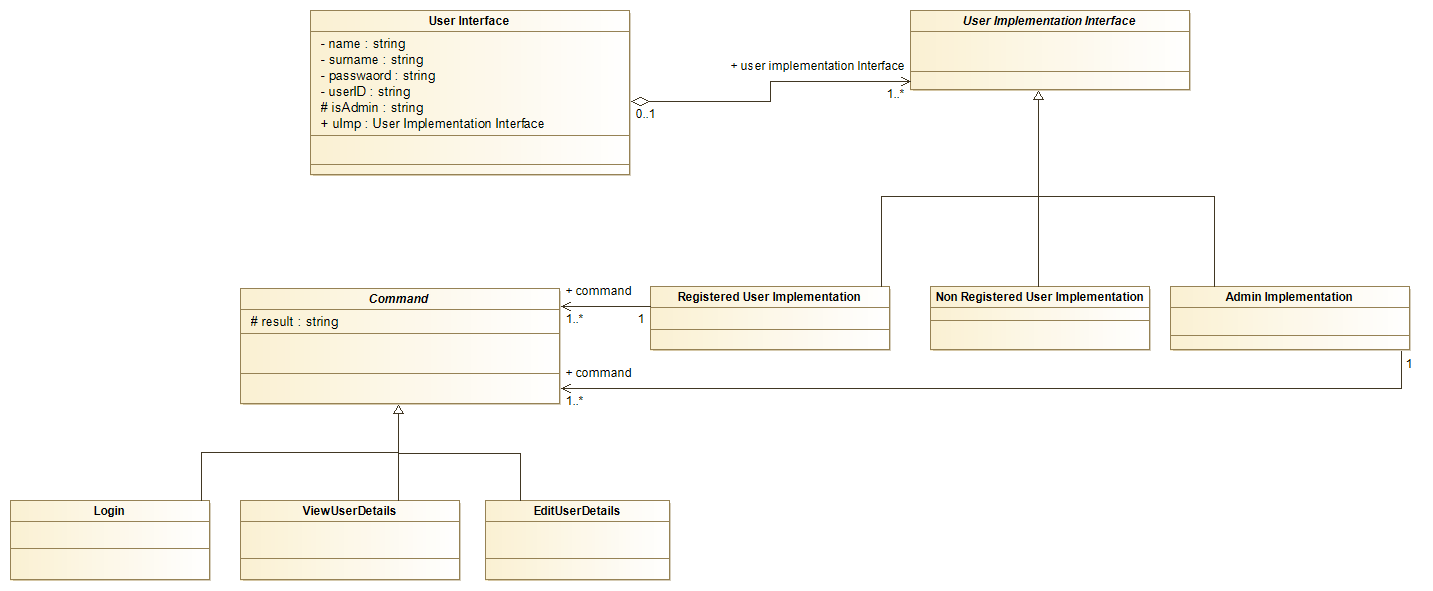
\includegraphics[width=12cm,height=26cm,keepaspectratio]{Users/Pictures/User_Class_Diagram.png}
	\caption{Class diagram for user management module}\label{visina8}
\end{figure}

\subsubsection{Sequence diagram}
\begin{figure}[H]
	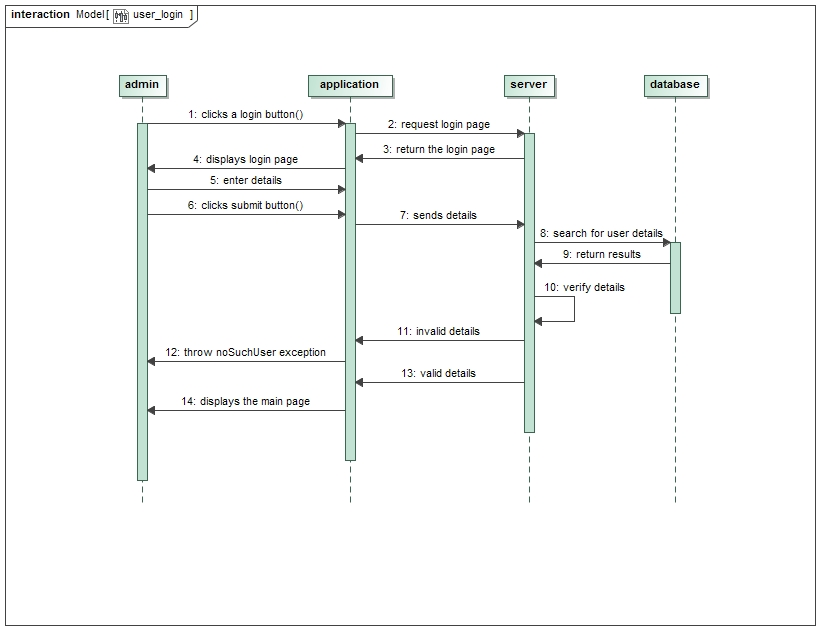
\includegraphics[width=12cm,height=26cm,keepaspectratio]{Users/Pictures/user_sequence_diagram.png}
	\caption{Sequence diagram for user management module}\label{visina8}
\end{figure}

\subsubsection{Activity diagram}
\begin{figure}[H]
	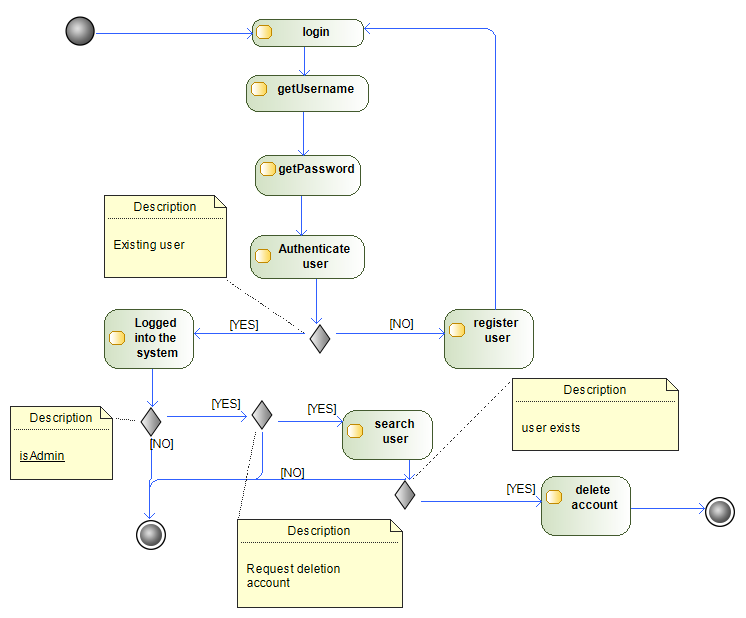
\includegraphics[width=12cm,height=26cm,keepaspectratio]{Users/Pictures/user_Activity_diagram.png}
	\caption{Activity diagram for user management module}\label{visina8}
\end{figure}
\subsubsection{State diagram}
\begin{figure}[H]
	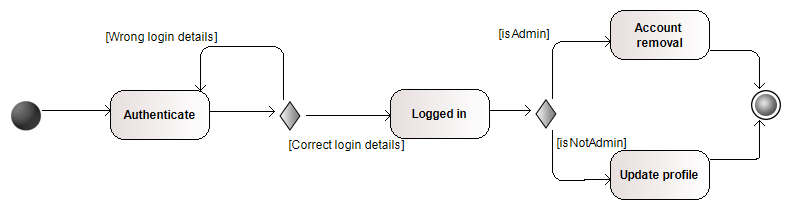
\includegraphics[width=12cm,height=26cm,keepaspectratio]{Users/Pictures/User_State_Diagram.png}
	\caption{State diagram for user management module}\label{visina8}
\end{figure}
\subsubsection{Use Case diagram}
\begin{figure}[H]
	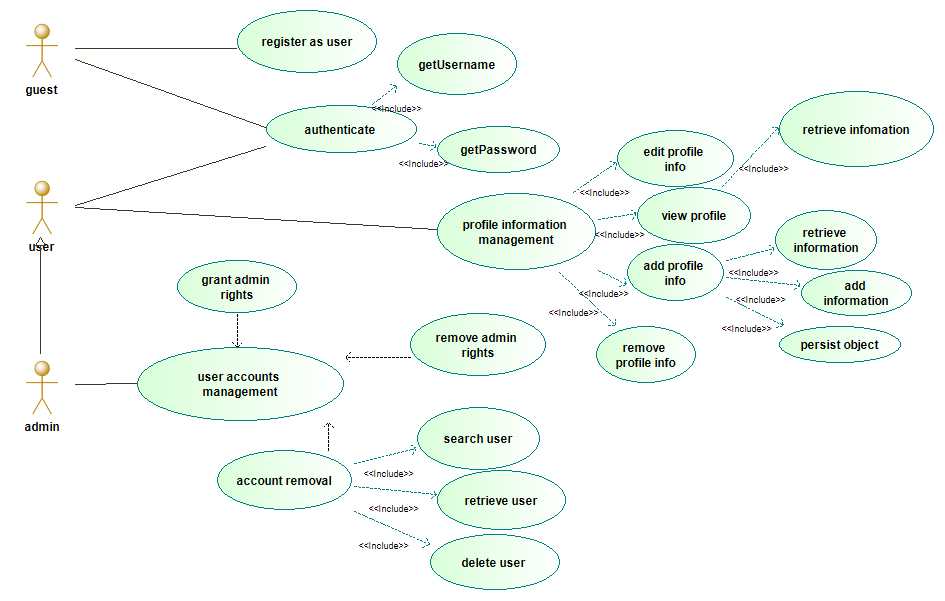
\includegraphics[width=12cm,height=26cm,keepaspectratio]{Users/Pictures/user_use_case_diagram.png}
	\caption{Use case diagram for user management module}\label{visina8}
\end{figure}

	
	\newpage
	
	\section{Technologies}
	For the NavUP system to be available to as many users as possible the system needs to be available on the two major mobile operating systems, iOS and Android as well as having a web interface. For the system to work on all three of these platforms we need a framework that works on all of these platforms. The main advantage of having only one framework that works on all three platforms is that it minimizes the amount of code required to make the app compatible with these three platforms. The latest distribution of Cordava, PhoneGap, fits this requirement well.
	
	\subsection{User Application}
	PhoneGap uses web technologies to create a front-end application for iOS and Android. Because web technologies are used the front-end code can be easily ported to be able to run on a browser. To improve the interface Angular.js and Express.js will be used. Cordova also have many open source plugins available on their website, these plugins make integration with the device's hardware simpler and also provide plugins that will make the implementation of some modules simpler as they have many of the functions these modules require.
	\subsection{Server}
	The server's operating system will be CentOS. CentOS is a very stable lightweight release of Linux and is primarily used for web servers. Most web hosting companies run their web servers on CentOS because of these reasons. The web server that will be used is Node.js. Node.js works best in real-time applications, because they work so well in real-time applications Node.js is perfect for the NavUP system which needs to provide real time data to the front-end application.
	\subsection{Database}
	We will use MongoDB as the database because it works well with NodeJS and is more secure than SQL.
	
	\subsection{Advantages and Disadvantages of Chosen Technologies}
	\begin{table}[H]
		\centering
		\resizebox{\textwidth}{!}{%
			\begin{tabular}{|l|l|}
				\hline
				\multicolumn{1}{|c|}{\textbf{Advantages}}                                                                                     & \textbf{Disadvantages}                                                                                                                                           \\ \hline
				\begin{tabular}[c]{@{}l@{}}PhoneGap works on all three required \\ platforms.\end{tabular}                                    & \begin{tabular}[c]{@{}l@{}}PhoneGap is not native to any of the \\ three platforms and performance can \\ sometimes be subdued.\end{tabular}                     \\ \hline
				PhoneGap is free.                                                                                                             & \begin{tabular}[c]{@{}l@{}}PhoneGap does not support all\\  functionality that might be needed.\end{tabular}                                                     \\ \hline
				Node.js is great for real time applications                                                                                   & \begin{tabular}[c]{@{}l@{}}Node.js isn’t consistent. It’s several, \\ development firms feel that the API \\ keeps enhancing at frequent intervals.\end{tabular} \\ \hline
				CentOS is perfect for web servers.                                                                                            & \begin{tabular}[c]{@{}l@{}}CentOS is not frequently updated and\\  therefore new software is not always \\ available.\end{tabular}                               \\ \hline
				\begin{tabular}[c]{@{}l@{}}JavaScript will be the main language used, \\ which will simplify the implementation.\end{tabular} & \begin{tabular}[c]{@{}l@{}}JavaScript can sometimes be slow to \\ execute.\end{tabular}                                                                          \\ \hline
			\end{tabular}%
		}
	\end{table}
	
\end{document}